\documentclass{article}
\usepackage[utf8]{inputenc}
\usepackage{amsmath}
\usepackage{amssymb}
\usepackage{graphicx}
\usepackage[english]{babel}

\setlength{\oddsidemargin}{0in}
\setlength{\textwidth}{6.5in}
\setlength{\topmargin}{-.55in}
\setlength{\textheight}{9in}
\pagestyle{empty}

\graphicspath{{Images/}}

\title{Scientific Computation HW3}
\author{Michael Nameika}
\date{September 2022}

\begin{document}

\maketitle

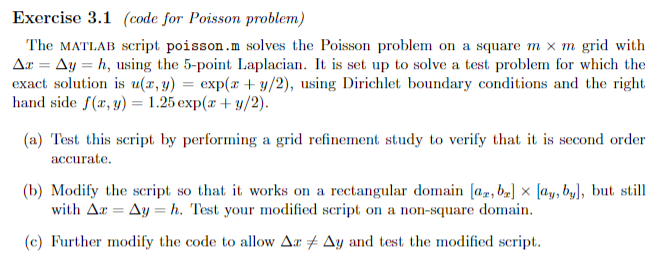
\includegraphics[scale = 0.8]{ex3.1.PNG}

(a) By introducing a for loop to loop through increasing values of $m$, ($m = 20, 40, 60, 80, 100$), and using the error\_table.m and error\_loglog.m files, we find the following:

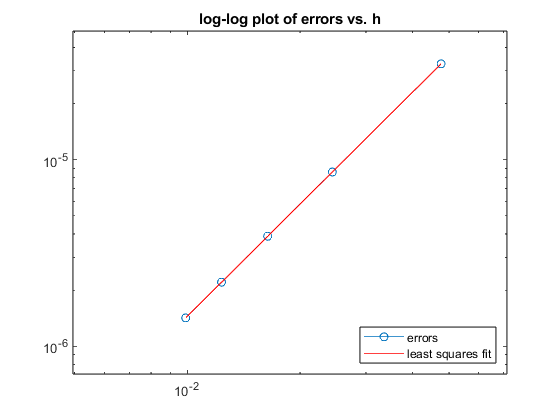
\includegraphics[scale = 0.5]{loglog_error_poisson.png}
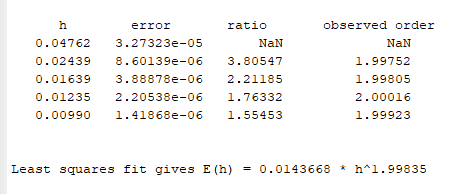
\includegraphics[scale = 0.7]{error_table_poisson.PNG}

which shows us the 5-point is approximately a second order method, which is what we wished to show.

(b) See the attached poisson\_rectangular\_Nameika.m for changes to poisson.m.
\newline
running the modified script results in the following:
\begin{center}
    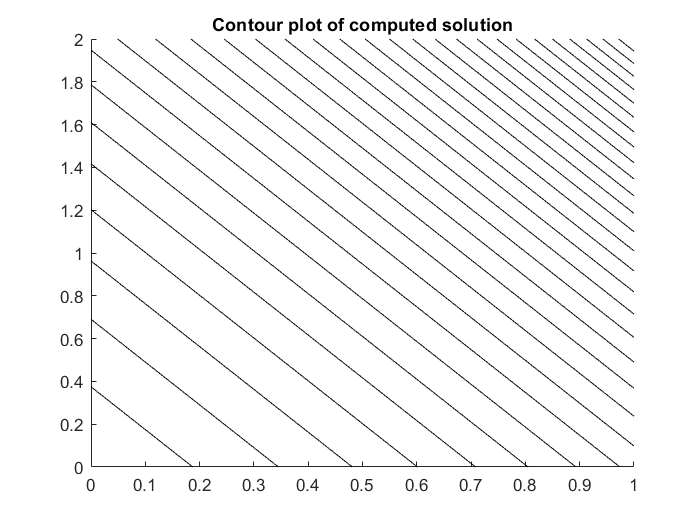
\includegraphics[scale = 0.6]{rectangulardomaingraph.png}
    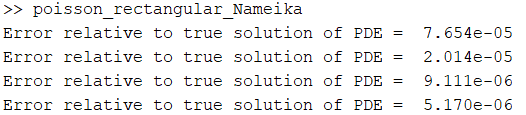
\includegraphics[scale = 0.8]{rectangulardomainerr.PNG}
\end{center}
as we can see, there is hardly any change in the error when decreasing the value of $h$. I suspect this may be due to the fact that $h$ is the same for both $x$ and $y$, which could lead to grid irregularities on a rectangular domain.

(c) For the case $\Delta y \neq \Delta x$, the five point method becomes
\[\frac{1}{(\Delta x)^2}(u_{i-1,j} + u_{i+1,j}) + \frac{1}{(\Delta y)^2}(u_{i,j-1} + u_{i,j-1}) - 2\left(\frac{1}{(\Delta x)^2} + \frac{1}{(\Delta y)^2}\right)u_{i,j} = f_{i,j}\]
Writing out the matrix $A$ using this equation, we find
\[A = \begin{bmatrix}
    T & Y & & & & \\
    Y & T & Y & & \\
     & \ddots & \ddots & \ddots & \\
     & & Y & T & Y\\
     
\end{bmatrix}\]
where
\[T = \begin{bmatrix}
    -2\left(\frac{1}{(\Delta x)^2} + \frac{1}{(\Delta y)^2}\right) & \frac{1}{(\Delta x)^2} & & &\\
    \frac{1}{(\Delta x)^2} & -2\left(\frac{1}{(\Delta x)^2} + \frac{1}{(\Delta y)^2}\right) & \frac{1}{(\Delta x)^2} & & \\
    & \frac{1}{(\Delta x)^2} & -2\left(\frac{1}{(\Delta x)^2} + \frac{1}{(\Delta y)^2}\right) & \frac{1}{(\Delta x)^2} & \\
    & & \ddots & \ddots & \ddots & \\
    & & & \frac{1}{(\Delta x)^2} & -2\left(\frac{1}{(\Delta x)^2} + \frac{1}{(\Delta y)^2}\right) & \frac{1}{(\Delta x)^2}\\
    
\end{bmatrix}\]
and
\[Y = \frac{1}{(\Delta y)^2}\begin{bmatrix}
    1 & & & \\
     & 1 & & \\
     & & \ddots & \\
     & & & 1\\
\end{bmatrix}\]
Modifying the code to implement this modification, we find the following:
\begin{center}
    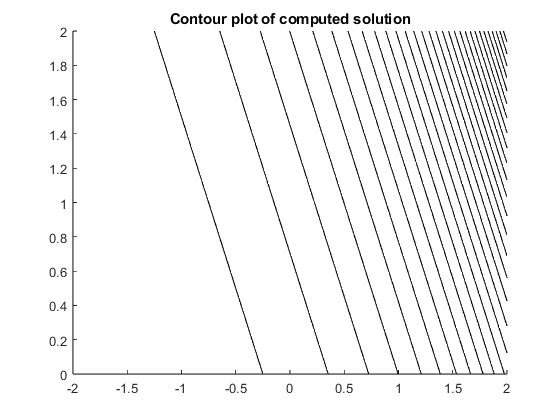
\includegraphics[scale = 0.6]{deltaydeltax.png}

    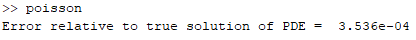
\includegraphics[scale = 0.8]{deltaydeltaxerror.PNG}
\end{center}
where we defined $\Delta y = \frac{b_y - a_y}{m + 1}$ and $\Delta x = \frac{b_x + a_x}{m + 1}$. Running the script for the rectangular domain we used in part (b) gives us
\begin{center}
    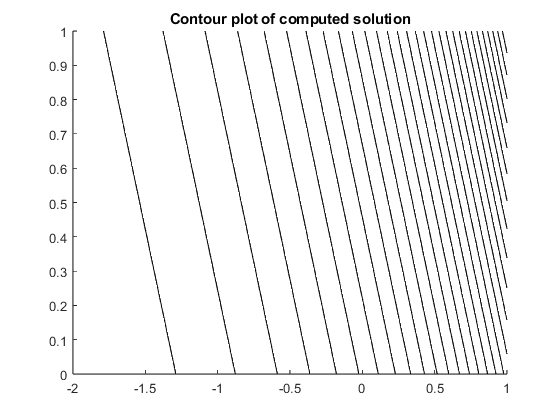
\includegraphics[scale = 0.6]{unevengrid.png}
    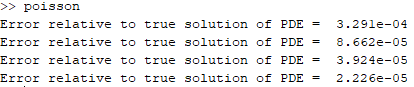
\includegraphics[scale = 0.8]{unevengriderr.PNG}
\end{center}
As we can see, the error has significantly improved from part (b). See the attached code file for precisely what changes were made to the script.
\newline


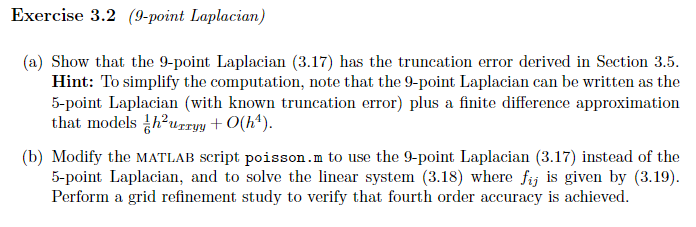
\includegraphics[scale = 0.8]{ex3.2.PNG}

(a) Using Taylor expansion (see page of work at the end of the document), we find the following:
\[\nabla^2_9 u_{ij} = \nabla^2 u_{ij} + \frac{h^2}{12}\left( \frac{\partial^4u_{ij}}{\partial x^4} + 2\frac{\partial^4u_{ij}}{\partial x^2 \partial y^2}  + \frac{\partial^4u_{ij}}{\partial y^4}\right) + \mathcal{O}(h^4) \]
Which is what we wanted to show.
\newline

(b) The nine point laplacian is given by the following formula:
\[\nabla^2_9 u_{ij} = \frac{1}{6h^2}(u_{i-1,j+1} + u_{i-1,j-1} + u_{i+1,j-1} + u_{i+1,j+1} + 4u_{i,j-1} + 4u_{i,j+1} + 4u_{i-1,j} + 4u_{i+1,j} - 20u_{ij})\]
Writing this in matrix form, we see
\[A = \frac{1}{6h^2}\begin{bmatrix}
    W & T & & & & & \\
    T & W & T & & & \\
     & T & W & T & & \\
     & & \ddots & \ddots & \ddots & \\
     & & & T & W & T\\
     & & & & T & W\\
\end{bmatrix}\]
where 
\[W = \begin{bmatrix}
    -20 & 4 & & & \\
    4 & -20 & 4 & & \\
     & 4 & -20 & 4 & \\
     & & \ddots & \ddots & \ddots\\
     & & & 4 & -20 & 4 \\
     & & & & 4 & -20 \\
\end{bmatrix}\]
is an $m \times m$ matrix where $m$ is the number of interior points in the $x$ dimension. And
\[T = \begin{bmatrix}
    4 & 1 & & & & \\
    1 & 4 & 1 & & & \\
     & 1 & 4 & 1 & & \\
     & & \ddots & \ddots & \ddots & \\
     & & & 1 & 4 & 1\\
     & & & & 1 & 4 \\ 
\end{bmatrix}\]
is an $n \times n$ matrix where $n$ is the number of interior points in the $y$ dimension. Implementing this change in the poisson.m script and accounting for the added boundary conditions introduced with the four extra points added by the nine point laplacian, we find the following on $[0,1] \times [0,1]$:

\begin{center}
`   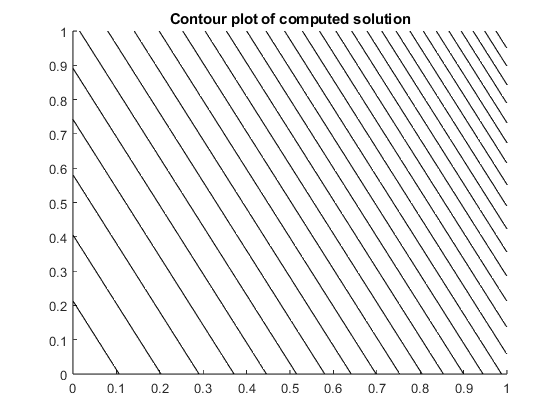
\includegraphics[scale = 0.6]{oh4table.png}
    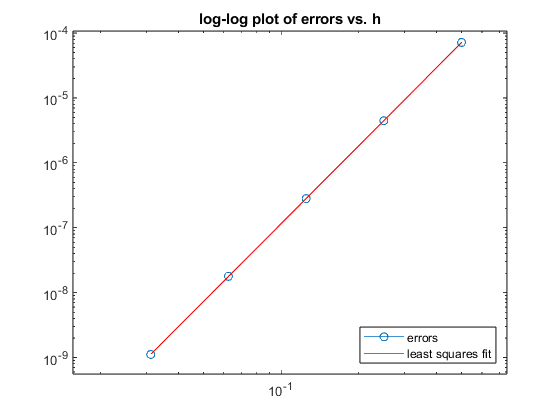
\includegraphics[scale = 0.45]{OH4BABY.png}
    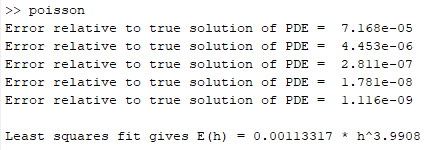
\includegraphics[scale = 0.8]{ayo.PNG}
\end{center}

Notice the changes made to the right hand side:
\begin{center}
    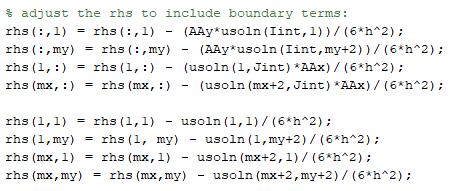
\includegraphics[scale = 0.9]{change.PNG}
\end{center}
Where $AAx$ is an $m\times m$ tridiagonal matrix with 1 on the super and sub diagonal and 4 on the main diagonal. Similarly, $AAy$ is an $n \times n$ tridiagonal matrix with 1 on the super and sub diagonal and 4 on the main diagonal.


See attached code file for more details.



\newpage
\section*{Work for 3.2 (a)}
To begin, recall Taylor's expansion for a smooth function of two variables centered at $(x_0, y_0)$:
\[f(x,y) = \sum_{i=0}^n\sum_{j=0}^{n-i} \frac{1}{i!j!}\frac{\partial^{i + j}f(x_0,y_0)}{\partial x^i \partial y^{j}}(x - x_0)^i(y - y_0)^j + \mathcal{O}(h^{n+1})\]
In our case, $x_0 = x_i$, $y_0 = y_j$ and $x_{i+1} = x_i + h$, $y_{j+1} = y_j + h$.
\newline
Now, let's find the Taylor expansion for $u_{i-1,j+1}, u_{i+1,j-1}, u_{i-1,j-1}, u_{i+1,j+1}, u_{i, j-1}, u_{i,j+1}, u_{i-1,j},$ and $u_{i+1,j}$:
\[u_{i-1,j} = u_{ij} - h\frac{\partial u_{ij}}{\partial x} + \frac{h^2}{2}\frac{\partial^2 u_{ij}}{\partial x^2} - \frac{h^3}{3!}\frac{\partial^3 u_{ij}}{\partial x^3} + \frac{h^4}{4!}\frac{\partial^4 u_{ij}}{\partial x^4} - \frac{h^5}{5!}\frac{\partial^5 u_{ij}}{\partial x^5} + \mathcal{O}(h^6)\]
\[u_{i+1,j} = u_{ij} + h\frac{\partial u_{ij}}{\partial x} + \frac{h^2}{2}\frac{\partial^2 u_{ij}}{\partial x^2} + \frac{h^3}{3!}\frac{\partial^3 u_{ij}}{\partial x^3} + \frac{h^4}{4!}\frac{\partial^4 u_{ij}}{\partial x^4} + \frac{h^5}{5!}\frac{\partial^5 u_{ij}}{\partial x^5} + \mathcal{O}(h^6)\]
then
\begin{equation}
    u_{i-1,j} + u_{i+1,j} = 2u_{ij} + h^2\frac{\partial^2 u_{ij}}{\partial x^2} + \frac{2h^4}{4!}\frac{\partial^4 u_{ij}}{\partial x^4} + \mathcal{O}(h^6)
\end{equation}
Similarly,
\[u_{i,j-1} = u_{ij} - h\frac{\partial u_{ij}}{\partial y} + \frac{h^2}{2}\frac{\partial^2 u_{ij}}{\partial y^2} - \frac{h^3}{3!}\frac{\partial^3 u_{ij}}{\partial y^3} + \frac{h^4}{4!}\frac{\partial^4 u_{ij}}{\partial y^4} - \frac{h^5}{5!}\frac{\partial^5 u_{ij}}{\partial y^5} + \mathcal{O}(h^6)\]
\[u{i,j+1} = u_{ij} + h\frac{\partial u_{ij}}{\partial y} + \frac{h^2}{2}\frac{\partial^2 u_{ij}}{\partial y^2} + \frac{h^3}{3!}\frac{\partial^3 u_{ij}}{\partial y^3} + \frac{h^4}{4!}\frac{\partial^4 u_{ij}}{\partial y^4} + \frac{h^5}{5!}\frac{\partial^5 u_{ij}}{\partial y^5} + \mathcal{O}(h^6)\]
Then
\begin{equation}
    u_{i, j-1} + u_{i, j+1} = 2u_{ij} + h^2\frac{\partial^2 u_{ij}}{\partial y^2} + \frac{2h^4}{4!}\frac{\partial^4 u_{ij}}{\partial y^4} + \mathcal{O}(h^6)
\end{equation}
Now,
\[u_{i-1,j-1} = u_{ij} - h\frac{\partial u_{ij}}{\partial x} - h\frac{\partial u_{ij}}{\partial y} + \frac{h^2}{2}\frac{\partial^2 u_{ij}}{\partial x^2} + \frac{h^2}{2}\frac{\partial^2 u_{ij}}{\partial y^2} - \frac{h^3}{3!}\frac{\partial^3 u_{ij}}{\partial x^3} - \frac{h^3}{3!}\frac{\partial^3 u_{ij}}{\partial y^3} - \frac{h^3}{2}\frac{\partial^3 u_{ij}}{\partial x^2 \partial y} - \frac{h^3}{2}\frac{\partial^3 u_{ij}}{\partial y^2 \partial x} + \frac{h^4}{4!}\frac{\partial^4 u_{ij}}{\partial x^4} + \]
\[ + \frac{h^4}{4!}\frac{\partial^4 u_{ij}}{\partial y^4} + \frac{h^4}{3!}\frac{\partial^4 u_{ij}}{\partial x^3 \partial y} + \frac{h^4}{3!}\frac{\partial^4 u_{ij}}{\partial x \partial y^3} + \frac{h^4}{4}\frac{\partial^4 u_{ij}}{\partial x^2 \partial y^2} - \frac{h^5}{5!}\frac{\partial^5 u_{ij}}{\partial x^5} - \frac{h^5}{5!}\frac{\partial^5 u_{ij}}{\partial y^5} - \frac{h^5}{4!}\frac{\partial^5 u_{ij}}{\partial x^4\partial y} - \frac{h^5}{4!}\frac{\partial^5 u_{ij}}{\partial x\partial y^4} - \frac{h^5}{3!}\frac{\partial^5 u_{ij}}{\partial x^3 \partial y^2} + \]
\[ - \frac{h^5}{3!}\frac{\partial^5 u_{ij}}{\partial x^2 \partial y^3} + \mathcal{O}(h^6)\]
Similarly,
\[u_{i+1,j+1} = u_{ij} - h\frac{\partial u_{ij}}{\partial x} + h\frac{\partial u_{ij}}{\partial y} + \frac{h^2}{2}\frac{\partial^2 u_{ij}}{\partial x^2} + \frac{h^2}{2}\frac{\partial^2 u_{ij}}{\partial y^2} + \frac{h^3}{3!}\frac{\partial^3 u_{ij}}{\partial x^3} + \frac{h^3}{3!}\frac{\partial^3 u_{ij}}{\partial y^3} + \frac{h^3}{2}\frac{\partial^3 u_{ij}}{\partial x^2 \partial y} + \frac{h^3}{2}\frac{\partial^3 u_{ij}}{\partial y^2 \partial x} + \frac{h^4}{4!}\frac{\partial^4 u_{ij}}{\partial x^4} + \]
\[ + \frac{h^4}{4!}\frac{\partial^4 u_{ij}}{\partial y^4} + \frac{h^4}{3!}\frac{\partial^4 u_{ij}}{\partial x^3 \partial y} + \frac{h^4}{3!}\frac{\partial^4 u_{ij}}{\partial x \partial y^3} + \frac{h^4}{4}\frac{\partial^4 u_{ij}}{\partial x^2 \partial y^2} + \frac{h^5}{5!}\frac{\partial^5 u_{ij}}{\partial x^5} - \frac{h^5}{5!}\frac{\partial^5 u_{ij}}{\partial y^5} - \frac{h^5}{4!}\frac{\partial^5 u_{ij}}{\partial x^4\partial y} + \frac{h^5}{4!}\frac{\partial^5 u_{ij}}{\partial x\partial y^4} + \frac{h^5}{3!}\frac{\partial^5 u_{ij}}{\partial x^3 \partial y^2} + \]
\[ + \frac{h^5}{3!}\frac{\partial^5 u_{ij}}{\partial x^2 \partial y^3} + \mathcal{O}(h^6)\]
Then

\begin{equation}
\begin{split}
    u_{i-1,j-1} + u_{i+1,j+1} &= 2u_{ij} + h^2\frac{\partial^2 u_{ij}}{\partial x^2} + h^2\frac{\partial^2 u_{ij}}{\partial y^2} + 2h^2\frac{\partial^2 u_{ij}}{\partial x \partial y} + \frac{2h^4}{4!}\frac{\partial^4 u_{ij}}{\partial x^4} + \frac{2h^4}{4!}\frac{\partial^4 u_{ij}}{\partial y^4} + \frac{h^4}{3}\frac{\partial^4 u_{ij}}{\partial x^3 \partial y} + \\
    & +  \frac{h^4}{3}\frac{\partial^4 u_{ij}}{\partial x \partial y^3} + \frac{h^4}{2} \frac{\partial^4 u_{ij}}{\partial x^2 \partial y^2} + \mathcal{O}(h^6)
    \end{split}
\end{equation}
Now,
\[u_{i-1,j+1} = u_{ij} - h\frac{\partial u_{ij}}{\partial x} + h\frac{\partial u_{ij}}{\partial y} + \frac{h^2}{2}\frac{\partial^2 u_{ij}}{\partial x^2} + \frac{h^2}{2}\frac{\partial^2 u_{ij}}{\partial y^2} - h^2\frac{\partial^2 u_{ij}}{\partial x \partial y} - \frac{h^3}{3!}\frac{\partial^3 u_{ij}}{\partial x^3} + \frac{h^3}{3!}\frac{\partial^3 u_{ij}}{\partial y^3} + \frac{h^3}{2}\frac{\partial^3 u_{ij}}{\partial x^2 \partial y} - \frac{h^3}{2}\frac{\partial^3 u_{ij}}{\partial x \partial y^2} + \frac{h^4}{4!}\frac{\partial^4 u_{ij}}{\partial x^4} + \]
\[+ \frac{h^4}{4!}\frac{\partial^4 u_{ij}}{\partial y^4} + \frac{h^4}{2}\frac{\partial^4 u_{ij}}{\partial x^2 \partial y^2} - \frac{h^4}{3!}\frac{\partial^4 u_{ij}}{\partial x \partial y^3} - \frac{h^3}{3!}\frac{\partial^4 u_{ij}}{\partial x^3 \partial y} - \frac{h^5}{5!}\frac{\partial^5 u_{ij}}{\partial x^5} + \frac{h^5}{5!}\frac{\partial^5 u_{ij}}{\partial y^5} + \]
\[- \frac{h^5}{4!}\frac{\partial^5 u_{ij}}{\partial x \partial y^4} + \frac{h^5}{5!}\frac{\partial^5 u_{ij}}{\partial x^4 \partial y} - \frac{h^5}{3!}\frac{\partial^5 u_{ij}}{\partial x^3 \partial y^2} + \frac{h^5}{3!}\frac{\partial u_{ij}}{\partial x^2 \partial y^3} + \mathcal{O}(h^6)\]
Similarly,
\[u_{i+1,j-1} = u_{ij} + h\frac{\partial u_{ij}}{\partial x} - h\frac{\partial u_{ij}}{\partial y} + \frac{h^2}{2}\frac{\partial^2 u_{ij}}{\partial x^2} + \frac{h^2}{2}\frac{\partial^2 u_{ij}}{\partial y^2} - h^2\frac{\partial^2 u_{ij}}{\partial x \partial y} + \frac{h^3}{3!}\frac{\partial^3 u_{ij}}{\partial x^3} - \frac{h^3}{3!}\frac{\partial^3 u_{ij}}{\partial y^3} - \frac{h^3}{2}\frac{\partial^3 u_{ij}}{\partial x^2 \partial y} + \frac{h^3}{2}\frac{\partial^3 u_{ij}}{\partial x \partial y^2} + \frac{h^4}{4!}\frac{\partial^4 u_{ij}}{\partial x^4} + \]
\[+ \frac{h^4}{4!}\frac{\partial^4 u_{ij}}{\partial y^4} + \frac{h^4}{2}\frac{\partial^4 u_{ij}}{\partial x^2 \partial y^2} - \frac{h^4}{3!}\frac{\partial^4 u_{ij}}{\partial x \partial y^3} - \frac{h^3}{3!}\frac{\partial^4 u_{ij}}{\partial x^3 \partial y} + \frac{h^5}{5!}\frac{\partial^5 u_{ij}}{\partial x^5} - \frac{h^5}{5!}\frac{\partial^5 u_{ij}}{\partial y^5} + \]
\[+ \frac{h^5}{4!}\frac{\partial^5 u_{ij}}{\partial x \partial y^4} - \frac{h^5}{5!}\frac{\partial^5 u_{ij}}{\partial x^4 \partial y} + \frac{h^5}{3!}\frac{\partial^5 u_{ij}}{\partial x^3 \partial y^2} - \frac{h^5}{3!}\frac{\partial^5 u_{ij}}{\partial x^2 \partial y^3} + \mathcal{O}(h^6)\]
Then
\begin{equation} 
    \begin{split}
     u_{i-1,j+1} + u_{i+1,j-1} &= 2u_{ij} + h^2\frac{\partial^2 u_{ij}}{\partial x^2} + h^2\frac{\partial^2 u_{ij}}{\partial y^2} - 2h^2\frac{\partial^2 u_{ij}}{\partial x \partial y} + \frac{2h^4}{4!}\frac{\partial^4 u_{ij}}{\partial x^4} + \frac{2h^4}{4!}\frac{\partial^4 u_{ij}}{\partial y^4} + \frac{h^4}{2}\frac{\partial^2 u_{ij}}{\partial x^2 \partial y^2} + \\
     & - \frac{2h^4}{3!}\frac{\partial^4 u_{ij}}{\partial x \partialy^3} - \frac{2h^4}{3!}\frac{\partial^4 u_{ij}}{\partial x^3 \partial y} +     \mathcal{O}(h^6)
    \end{split}
\end{equation}
Finally, adding up $\frac{1}{6h^2}(4u_{i-1,j} + 4u_{i+1,j} + 4u_{i,j-1} + 4u_{i,j+1} + u_{i-1,j-1} + u_{i-1,j+1} + u_{i+1,j-1} + u_{i+1,j+1} - 20u_{ij})$, we find
\[\nabla_9^2 u_{ij} = \frac{1}{6h^2}\left( 6h^2\nabla^2u_{ij} + \frac{h^4}{2}\left(\frac{\partial^4u_{ij}}{\partial x^4} + 2\frac{\partial^4u_{ij}}{\partial x^2 \partial y^2} + \frac{\partial^4 u_{ij}}{\partial y^4}\right) +\mathcal{O}(h^6) \right)\]
\[ = \nabla^2 u_{ij} + \frac{h^2}{12}\left( \frac{\partial^4u_{ij}}{\partial x^4} + 2\frac{\partial^4u_{ij}}{\partial x^2 \partial y^2} + \frac{\partial^4 u_{ij}}{\partial y^4} \right) + \mathcal{O}(h^4)\]

\end{document}
